\documentclass[12pt]{article}
\usepackage{fullpage}
\usepackage{minted}
\usepackage{enumitem}
\usepackage{tikz}
\usetikzlibrary{shapes.multipart}
\title{Data Structures Problem Set \#2}
\author{Nicholas Yang}
\date{25 September 2017}
\begin{document}
\maketitle
\section{Problem 1}
\begin{enumerate}[label=(\alph*)]
\item
  First add a boolean for recomputing the area:
  \begin{minted}{Java}
    private boolean hasRadiusChanged;
  \end{minted}
\item Make sure to initialize it in the constructor:
  \begin{minted}{Java}
    public Circle(double centerX, double centerY, double radius) {
        center = new Point(centerX, centerY);
        this.radius = radius;
        boundingBox = new Rect(
            centerX - radius,
            centerX + radius,
            centerY - radius,
            centerY + radius
        );
        hasRadiusChanged = true;
    }
  \end{minted}
\item Then the setRadius method:
  \begin{minted}{Java}
    public void setRadius(double radius) {
        if (this.radius != radius) {
            hasRadiusChanged = true;
            this.radius = radius;
        }
    }
  \end{minted}
\item  Finally the area method:
  \begin{minted}{Java}
    public double area() {
        if (hasRadiusChanged) {
            area = Math.PI * radius * radius;
            hasRadiusChanged = false;
        }
        return area;
    }
  \end{minted}
\end{enumerate}
\section{Problem 2}
Stack visualization: \\[12pt]
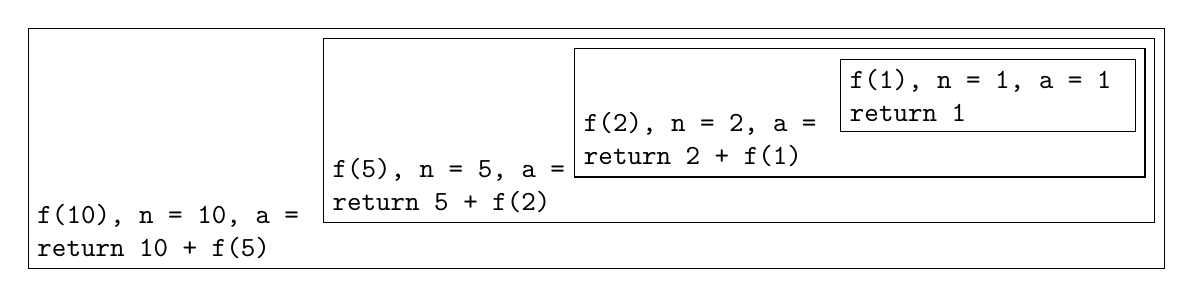
\begin{tikzpicture}[
    single/.style={draw, align=left, anchor=text, rectangle split, rectangle split parts=1},
  ]
  \node[single] {
    {\tt f(10), n = 10, a = }
    \tikz{
      \node[single] {
        {\tt f(5), n = 5, a =}
        \tikz{
          \node[single] {
            {\tt f(2), n = 2, a = }
            \tikz{
              \node[single] {
                {\tt f(1), n = 1, a = 1 } \\
                {\tt return 1}
              }
            } \\
            {\tt return 2 + f(1) }
          }
        } \\
        {\tt return 5 + f(2) }
      };
    } \\
    {\tt return 10 + f(5) }
  };
\end{tikzpicture} \\[12pt]
Or for the sum:
\begin{minted}{Python}
  f(10) = 10 + f(5)
        = 10 + 5 + f(2)
        = 10 + 5 + 2 + f(1)
        = 10 + 5 + 2 + 1
        = 18
\end{minted}
\section{Problem 3}
\begin{enumerate}[label=(\alph*)]
\item Write an interface {\tt ReduceFun } that has one abstract method {\tt int f(int a, int b)}:
  \begin{minted}{Java}
    public interface ReduceFun {
        int f(int a, int b);
    }
  \end{minted}
\item Write three classes that instantiate {\tt ReduceFun } and that override
  {\tt f} with methods that instantiate the above three functions {\tt p, q, r}:
  \begin{minted}{Java}
    public class SumReduce implements ReduceFun {
        public int f(int a, int b) {
            // p function
            return a + b;
        }
    }
    public class ProductReduce implements ReduceFun {
        public int f(int a, int b) {
            // q function
            return a * b;
        }
    }
    // Not the most accurate name, but DoubleAndDiffReduce seemed too clunky
    public class DifferenceReduce implements ReduceFun {
        public int f(int a, int b) {
            // r function
            return 2 * b - a;
        }
    }
  \end{minted}
\item Write a static method {\tt int reduceList(ReduceFun w, IntList l) } which returns the
  reduction of {\tt l} by {\tt w}:
  \begin{minted}{Java}
    public static int reduceList(ReduceFun w, IntList l) {
        // Renamed for clarity
        IntList node = l;
        // Start the accumulator with the first value.
        // Could be a NullPointerException, but that's
        // the fault of the caller
        int acc = node.getValue();
        while (node.getNext() != null) {
            // Immediately go to next node because
            // otherwise you'd repeat the first value
            node = node.getNext();
            acc = w.f(acc, node.getValue());
        }
        return acc;
    }
  \end{minted}
\item Write a small main function which is a driver illustrating the use of all this:
  \begin{minted}{Java}
    public static void main(String[] args) {
        SumReduce sumReduce = new SumReduce();
        ProductReduce productReduce = new ProductReduce();
        DifferenceReduce differenceReduce = new DifferenceReduce();
        // Create an IntList. No need to add a next node right now
        IntList myList = new IntList(10, null);
        int[] array = { 1, 2, 5, 8, 4, 11, 21, 4, 18 };
        // Add items to list
        for ( int item : array ) {
            myList.addEnd(item);
        }
        int sum = reduceList(sumReduce, myList);
        System.out.println(sum);
        int product = reduceList(productReduce, myList);
        System.out.println(product);
        int difference = reduceList(differenceReduce, myList);
        System.out.println(difference);
    }
  \end{minted}
\end{enumerate}
\section{Problem 4}
\begin{enumerate}
\item Define an abstract class {\tt Reducer } that has
  \begin{enumerate}[label=(\alph*)]
  \item An abstract method {\tt int f(int x, int y)}
  \item A concrete method {\tt int reduce(IntList l)} that reduces list {\tt l}
    using the method {\tt f(x, y) }
  \end{enumerate}
  \begin{minted}{Java}
    abstract class Reducer {
        abstract int f(int x, int y);
        
        public int reduce(IntList l) {
            // Renamed for clarity
            IntList node = l;
            // Start the accumulator with the first value.
            // Could be a NullPointerException, but that's
            // the fault of the caller
            int acc = node.getValue();
            while (node.getNext() != null) {
                // Immediately go to next node because
                // otherwise you'd repeat the first value
                node = node.getNext();
                acc = f(acc, node.getValue());
            }
            return acc;
        }
    }
  \end{minted}
\item Three concrete classes that extend {\tt Reducer } and that override {\tt
  f} with methods instantiating the above three functions {\tt p, q, r}
  \begin{minted}{Java}
    public class SumReducer extends Reducer {
        public int f(int x, int y) {
            // p function
            return x + y;
        }
    }
    public class ProductReducer extends Reducer {
        public int f(int x, int y) {
            // q function
            return x * y;
        }
    }
    public class DifferenceReducer extends Reducer {
        public int f(int x, int y) {
            return 2 * y - x;
        }
    }
  \end{minted}
\item A small main function that is a driver
  \begin{minted}{Java}
    public static void main(String[] args) {
        SumReducer sumReducer = new SumReducer();
        ProductReducer productReducer = new ProductReducer();
        DifferenceReducer differenceReducer = new DifferenceReducer();
        IntList myList = new IntList(10, null);
        int[] array = { 1, 2, 5, 8, 4, 11, 21, 4, 18 };
        for ( int item : array ) {
            myList.addEnd(item);
        }
        int sum = sumReducer.reduce(myList);
        System.out.println(sum);
        int product = productReducer.reduce(myList);
        System.out.println(product);
        int difference = differenceReducer.reduce(myList);
        System.out.println(difference);
    }
    \end{minted}
\end{enumerate}
\end{document}
